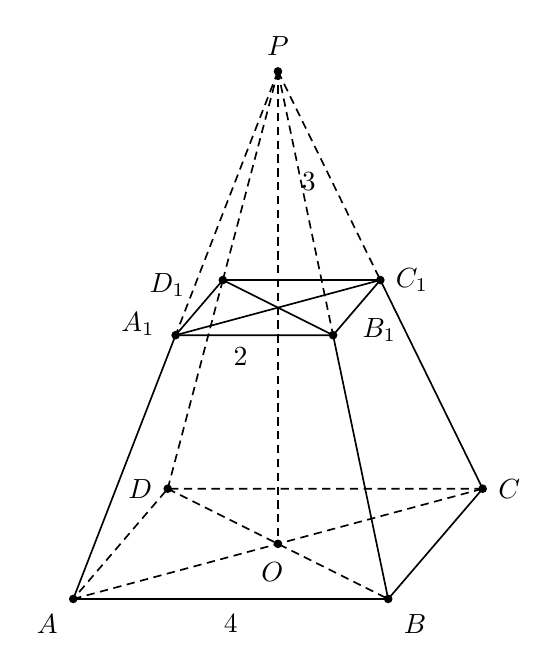
\begin{tikzpicture}[x=1cm,y=1cm,line width=.6pt]
\tikzset{pt/.style={circle,fill=black,inner sep=1.1pt}}
% frustum pyramid P-O, bottom half-side 2, top half-side 1
\coordinate (P) at (0.6000000000,6.0000000000);
\coordinate (O) at (0.6000000000,0.0000000000);
\coordinate (Ot) at (0.6000000000,3.0000000000);
\coordinate (A) at (-2,-0.7);
\coordinate (B) at (2,-0.7);
\coordinate (C) at (3.2000000000,0.7000000000);
\coordinate (D) at (-0.8000000000,0.7000000000);
\coordinate (A1) at (-0.7000000000,2.6500000000);
\coordinate (B1) at (1.3000000000,2.6500000000);
\coordinate (C1) at (1.9000000000,3.3500000000);
\coordinate (D1) at (-0.1000000000,3.3500000000);
% base
\draw[black] (A)--(B)--(C);
\draw[black,densely dashed] (C)--(D)--(A);
\draw[black,densely dashed] (A)--(O)--(C);
\draw[black,densely dashed] (D)--(O)--(B);
% top base solid + diagonals
\draw[black] (A1)--(B1)--(C1)--(D1)--cycle;
\draw[black] (A1)--(C1);
\draw[black] (D1)--(B1);
% laterals
\draw[black] (A)--(A1);
\draw[black] (B)--(B1);
\draw[black] (C)--(C1);
\draw[black,densely dashed] (D)--(D1);
% apex extensions + height
\draw[black,densely dashed] (P)--(A1);
\draw[black,densely dashed] (P)--(B1);
\draw[black,densely dashed] (P)--(C1);
\draw[black,densely dashed] (P)--(D1);
\draw[black,densely dashed] (P)--(O);
% dots
\foreach \p in {P,O,A,B,C,D,A1,B1,C1,D1}{\node[pt] at (\p) {};}
% point labels with clearance
\node[above=2pt] at (P) {$P$};
\node[below=3pt,xshift=-2pt] at (O) {$O$};
\node[below left=2pt] at (A) {$A$};
\node[below right=2pt] at (B) {$B$};
\node[right=2pt] at (C) {$C$};
\node[left=2pt] at (D) {$D$};
\node[left=2pt,xshift=-2pt,yshift=4pt] at (A1) {$A_{1}$};
\node[right=2pt,xshift=5pt,yshift=2pt] at (B1) {$B_{1}$};
\node[right=2pt] at (C1) {$C_{1}$};
\node[below=3pt,xshift=-1pt,xshift=-19.071pt,yshift=9.034pt] at (D1) {$D_{1}$};
% size labels offset from PO to avoid touching
\node[right=5pt] at (.6,4.6) {$3$};
\node[below=2pt,xshift=-5pt,yshift=1pt] at (.3,2.65) {$2$};
\node[below=2pt] at (0,-0.7) {$4$};
\end{tikzpicture}

